\documentclass{article}

\usepackage{listings}
\usepackage{xcolor}
\usepackage{caption}
\usepackage[a4paper, total={6in, 10in}]{geometry}
\usepackage[utf8x]{inputenc}
\usepackage[framemethod=tikz]{mdframed}

\lstset{
  language=C,               
  numbers=left,             
  stepnumber=1,             
  numbersep=10pt,           
  backgroundcolor=\color{white},
  showspaces=false,             
  showtabs=false,               
  tabsize=2,                    
  captionpos=b,                 
  breaklines=true,              
  breakatwhitespace=true,       
  belowcaptionskip=1\baselineskip,
  breaklines=true,
  xleftmargin=\parindent,
  showstringspaces=false,
  basicstyle=\footnotesize\ttfamily,
  keywordstyle=\bfseries\color{blue!40!black},
  commentstyle=\itshape\color{green!40!black},
  stringstyle=\color{orange},
}

\newcommand\mylstcaption{}

\mdfdefinestyle{mymdstyle}{
hidealllines=true,
middleextra={
  \node[anchor=west] at (O|-P)
    {\lstlistingname~\thelstlisting\  (Cont.):~\mylstcaption};},
secondextra={
  \node[anchor=west] at (O|-P)
    {\lstlistingname~\thelstlisting\  (Cont.):~\mylstcaption};},
splittopskip=2\baselineskip
}

\surroundwithmdframed[style=mymdstyle]{lstlisting}
\newmdenv[style=mymdstyle]{mdlisting}

\begin{document}
\section{Writing a simple concurrent caching http proxy}
\paragraph{Solution}
The created proxy is a simple implementation of a forward proxy.
It supports only HTTP GET request. But allow for multiple clients to be served concurrently.
Also, it supports response caching with least recently used (LRU) cache policy.
It uses two additional custom C modules \textsf{sbuf} and \textsf{cache}:
\begin{itemize}
    \item The \textsf{sbuf} is a simple implementation of a concurrent producer/consumer buffer.
It uses semaphores to limit the number of readers and writers based on available item slots.
And an exclusive lock for accessing buffered items.
    \item The \textsf{cache} is an LRU cache, with linked list cache structure.
LRU is provided by maintaining a linked list queue for access history.
It moves cache item access record to the end of the queue each time the item is accessed.
When total cache size becomes greater than the limit, 
it evicts item with LRU records located at the beginning of the LRU queue.
\end{itemize}
The source code of proxy is shown on listing \ref{lst:c1}, 
the source code of sbuf and cache is shown on listing \ref{lst:c2} 
and listing \ref{lst:c3} correspondingly.
\renewcommand\mylstcaption{proxy.c}
\begin{mdlisting}
    \lstinputlisting[caption=\mylstcaption, label=lst:c1]{../proxy.c}
\end{mdlisting}
\newpage
\renewcommand\mylstcaption{sbuf.c}
\begin{mdlisting}
    \lstinputlisting[caption=\mylstcaption, label=lst:c2]{../sbuf.c}
\end{mdlisting}
\newpage
\renewcommand\mylstcaption{cache.c}
\begin{mdlisting}
    \lstinputlisting[caption=\mylstcaption, label=lst:c3]{../cache.c}
\end{mdlisting}
\paragraph{Results}
The proxy was run against the evaluator which verifies basic requirements. 
\begin{itemize}
    \item Validity of the proxy response. Figure \ref{fig:basic}.
    \item Support of concurrent requests. Figure \ref{fig:concurrency}.
    \item And functionality of the caching policy. Figure \ref{fig:cache}.
\end{itemize}
\begin{figure}[h]
    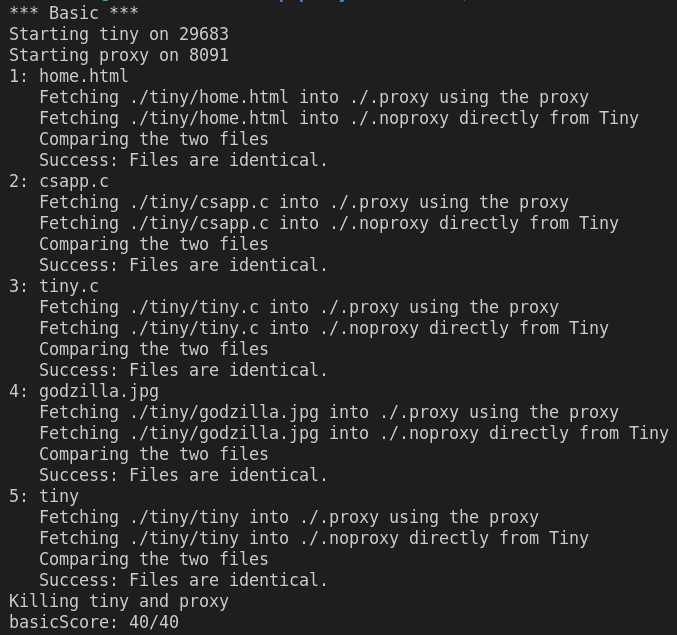
\includegraphics[width=0.6\textwidth]{basic.jpg}
    \centering
    \caption{Basic validity check}
    \label{fig:basic}
\end{figure}
\begin{figure}[h]
    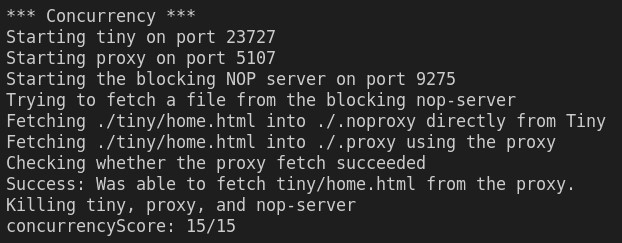
\includegraphics[width=0.6\textwidth]{concurrency.jpg}
    \centering
    \caption{Concurrency check}
    \label{fig:concurrency}
\end{figure}
\begin{figure}[h]
    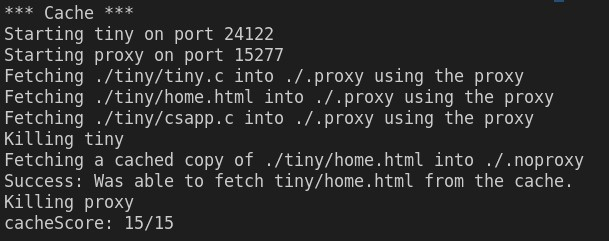
\includegraphics[width=0.6\textwidth]{cache.jpg}
    \centering
    \caption{Cache check}
    \label{fig:cache}
\end{figure}
\end{document}